
\documentclass[12pt,a4paper]{article}

\usepackage[margin=2.5cm]{geometry}

\usepackage{amsmath}
\usepackage{amsthm}
\newtheorem{theorem}{Theorem}[section] \newtheorem{proposition}[theorem]{Proposition} \newtheorem{lemma}[theorem]{Lemma} \newtheorem{corollary}[theorem]{Corollary} \theoremstyle{definition} \newtheorem{definition}[theorem]{Definition}
\theoremstyle{remark} \newtheorem{remark}[theorem]{Remark}


\usepackage{amssymb}
\usepackage{amsfonts}
\usepackage{array}
\usepackage{listings}
\usepackage{xcolor}

\lstdefinestyle{pythonstyle}{
    language=Python,
    basicstyle=\ttfamily\small,
    frame=single,
    breaklines=true,
    showstringspaces=false,
    numbers=left,
    numberstyle=\tiny,
    captionpos=b
}

\usepackage{graphicx}
\usepackage{mathrsfs}
\usepackage{multirow}
\usepackage{siunitx}
\usepackage{algorithm}
\usepackage{algpseudocode}

\usepackage{float}
\usepackage{subcaption}

\newcounter{questioncounter}
\newcounter{equestioncounter}

\setlength{\parskip}{10pt}
\setlength{\parindent}{0in}

\newcommand{\bea}{\begin{eqnarray*}}
\newcommand{\eea}{\end{eqnarray*}}
\newcommand{\beao}{\begin{eqnarray}}
\newcommand{\eeao}{\end{eqnarray}}
\newcommand{\no}{\noindent}



\begin{document}
\title{Deep Learning in Rough Volatility Models}

\author{\fontsize{11.5}{13.5}\selectfont
Akmal Abu Bakar, Federico La Penna,
Aidan McDougall, Benjamin Kolicic\\[0.4em]
\small\textit{
\parbox{0.9\textwidth}{
\centering
Department of Mathematics, London School of Economics and Political Science, London, UK
}}
}

\date{}
\maketitle

\begin{abstract}
\noindent This project builds on the deep calibration framework for rough volatility models proposed by Horvath, Muguruza, and Tomas (2019) \cite{1}. As a first goal, the project shows how rough volatility models can be efficiently simulated in such a way as to overcome the high-variance structure of Monte Carlo estimators. Then, the focus moves to the efficiency of the deep calibration implementation and presents a practical two-step feed-forward neural network (FNN) learning procedure (offline learning and online calibration) that permits the routine to be used efficiently. Finally, the practical case of digital barrier option pricing is also addressed.



\end{abstract}

\section{Introduction}

The calibration of stochastic volatility models is a fundamental inverse problem in quantitative finance. Classical, Markovian stochastic volatility models such as Heston and SABR provide fast, tractable pricing that can be used for industrial applications. However, the volatility surfaces generated by these models are inconsistent with market observations.

Rough volatility models represent a fundamentally different class. Motivated by the empirical finding of Gatheral, Jaisson, and Rosenbaum (2018) \cite{gatheral} that the realised volatility of equity indices behaves as a fractional Brownian motion with Hurst parameter $H\approx 0.1$, these models replace the classical Markovian variance dynamics with a Volterra process driven by a singular kernel $(t-s)^{H-1/2}$. This rough structure reproduces the steep short-maturity skew observed in equity markets and provides a more accurate description of market dynamics. However, the non-Markovian nature of the variance process rules out many of the classical fast pricing approaches usually employed. Since each volatility surface to be evaluated requires tens of thousands of simulated paths, the calibration of rough volatility models becomes computationally prohibitive for industrial use.

Horvath et al. \cite{1} propose a way to overcome the problem through a two-step deep learning approach. In the first step, a feed-forward neural network is trained offline to approximate the pricing map from model parameters to implied volatility surfaces, using Monte Carlo-generated data as training labels, such that, once trained, the network replaces the slow simulator entirely. In the second step, the frozen network serves as a fast direct map to be calibrated online via classical gradient-based optimisation. The result is a calibration procedure that matches the accuracy of full Monte Carlo while operating at millisecond speed.\vspace{1em}\\

This project replicates the core findings of Horvath et al.\ \cite{1} and develops the theory underpinning them. After reviewing the preliminaries on neural networks and rough volatility models, Section~\ref{deep calibration chapter} formalises the calibration problem and the two-step framework that organises the rest of the report. Section~\ref{approximate pricing map} carries out the first step: it prices rough Bergomi financial contracts by Monte Carlo and trains the network that approximates the resulting pricing map. Section~\ref{calibration chapter} carries out the second, calibrating the trained map to market data.
\section{Preliminaries}
In this section we introduce the relevant theory needed to address the deep calibration of rough volatility models: feed-forward neural networks and the rough volatility models themselves.
\subsection{Neural networks}\label{neural networks section}
\begin{definition}[feed-forward neural network]
    A feed-forward neural network with $L-1$ hidden layers is a function $f:\mathbb R^{N_0}\to \mathbb R^{N_L}$ of the form
    \[
    f=\phi _L\circ A_L\circ\cdots\circ\phi _1\circ A_1
    \]
    where for $i\in \{1, ..., L-1\}$, $N_i\geq 1$ are the number of nodes in the $i^{th}$ layer; $\phi_i:\mathbb R^{N_i}\to \mathbb R^{N_i}$ is the activation function and $A_i:\mathbb R^{N_{i-1}}\to \mathbb R^{N_i}$ is the affine map composed of weights and a bias. The set of all such functions $f$ is denoted as $\mathcal N\mathcal N_{L}(N_0, N_1, ..., N_L, \phi_1, ..., \phi_L)$.
\end{definition}
\begin{theorem}[Hornik, Stinchcombe and White]
    Let $f\in C^n$, $g : \mathbb R^{N_0} \to \mathbb R$ and $\mathcal N\mathcal N(N_0, 1, \phi )$ be the set of single-layer neural networks with
activation function $\phi:\mathbb R\to \mathbb R$. Then, if the
(non-constant) activation function is $\phi\in C^{n}$, then $g\in \mathcal N\mathcal N(N_0, 1, \phi)$ arbitrarily approximates $f$ and all
its derivatives up to order $n$.
\end{theorem}
\noindent The above theorem is the universal approximation theorem for derivatives 
and provides the crucial theoretical foundation for the neural network that will be
constructed. The function to be approximated is the map $
F^* \colon \Theta \to\mathbb{R}^{d}$,
which maps the model parameters to the corresponding implied volatilities. 
Since gradient-based calibration requires an accurate approximation of
\(\nabla_{\theta} F^*\), the above theorem requires, at a minimum, an activation 
function \(\phi \in C^1(\mathbb{R})\).
Indeed, later on, the network will be constructed with the ELU activation function,
$\displaystyle \phi_{\mathrm{ELU}}(x)
=
\begin{cases}
x, & x > 0,\\
\alpha\left(e^x - 1\right), & x \leq 0.
\end{cases}$, which belongs to \(C^1(\mathbb{R})\) and 
therefore satisfies the requirement. Consequently, the neural network would 
approximate both the pricing map and its derivatives $
\nabla_{\theta}\widetilde{F}
\approx
\nabla_{\theta}F^*$.

\subsection{Rough volatility models}
Rough volatility models are a class of non-Markovian stochastic volatility models that incorporate a Volterra kernel into their dynamics, characterising their roughness behaviour. In finance, it is now well established that ``volatility is rough'' (Gatheral et al. \cite{gatheral}) and that financial assets exhibit volatility paths that differ fundamentally from classical Markovian structures such as the Heston model. The introduction of Volterra kernels gives rise to processes sharing the local regularity of fractional Brownian motion, whose characteristic roughness depends on the Hurst parameter ($H \in (0,1)$), with empirical studies finding ($H \approx 0.1$) for equity volatility.
\subsubsection{Rough Bergomi model}
\begin{definition}[Rough Bergomi model]
    On a filtered probability space $(\Omega, \mathcal F,(\mathcal F_t)_{t\geq 0}, \mathbb P)$ the Rough Bergomi model dynamic is defined by 
    \begin{align}
        dX_t&=-\frac{1}{2}V_tdt+\sqrt V_t dB_t, \quad X_0=0\label{logprice}\\
        V_t&= \xi_0(t)  \mathcal E(\sqrt{2H}\nu\int_0^t(t-s)^{H-1/2}dW_s ), \quad V_0=v_0>0\label{var rb}
    \end{align}
    Where $H\in (0,1)$ is the Hurst parameter, $\nu>0$ is the volatility-of-volatility, $\mathcal E(\cdot)$ is the stochastic exponential, $\xi_0$ denotes the forward variance curve, and $B, W$ are two Brownian motions with correlation $\rho\in[-1,1]$. $dX_t$ refers to the log-price SDE and $V_t$ is called the variance process.
        
\end{definition}
\noindent The roughness in the model enters through the variance process, which depends directly on the Volterra kernel $\displaystyle \int_0^t(t-s)^{H-1/2}dW_s$.


\section{Deep calibration}\label{deep calibration chapter}
Having introduced neural networks and rough volatility models, we now formalise the calibration problem they serve and present the two-step deep-calibration framework that organises the remainder of this report.

\subsection{The calibration problem}\label{calibration problem section}
In plain terms, calibration chooses the model parameters so that the model reproduces the observed market as closely as possible. To state this precisely, let $\mathcal M:=\mathcal M(\theta)_{\theta\in\Theta}$ be a model with parameter vector $\theta\in\Theta\subset\mathbb R^n$. The model and its parameters together fix the prices of any contracts written on the underlying. Let $\zeta$ denote those contracts, for instance vanilla options across a set of strikes and maturities, and let the \emph{pricing map}
\[
P:\mathcal M(\theta,\zeta)\to\mathbb R^m,\qquad m\in\mathbb N,
\]
return their model prices, with $\mathcal P^{\mathrm{MKT}}(\zeta)\in\mathbb R^m$ the corresponding market quotes. Given a metric $\delta(\cdot,\cdot)$ on $\mathbb R^m$, the parameter vector $\hat\theta$ solves the \emph{ideal $\delta$-calibration problem} if
\begin{equation}\label{ideal calibration}
\hat\theta=\operatorname*{argmin}_{\theta\in\Theta}\;\delta\!\left(P(\mathcal M(\theta),\zeta),\,\mathcal P^{\mathrm{MKT}}(\zeta)\right),
\end{equation}
with $\delta$ chosen to suit the contract $\zeta$ at hand.

For most models, and for \emph{every} rough volatility model, the pricing map $P$ has no closed form and must be replaced by a numerical scheme $\widetilde P$. Substituting it into \eqref{ideal calibration} gives the \emph{approximate $\delta$-calibration problem}: $\hat\theta\in\Theta$ solves it if
\begin{equation}\label{approx calibration}
\hat\theta=\operatorname*{argmin}_{\theta\in\Theta}\;\delta\!\left(\widetilde P(\mathcal M(\theta),\zeta),\,\mathcal P^{\mathrm{MKT}}(\zeta)\right).
\end{equation}
This is the problem we actually solve.

Replacing $P$ by Monte Carlo carries two costs. The first is \emph{speed}. For rough Bergomi the only available $\widetilde P$ is the Monte Carlo pricer of Section~\ref{rough bergomi chapter}, and calibration is iterative: every optimiser step re-evaluates $\widetilde P$, so a slow per-evaluation cost compounds over the whole optimisation and makes \eqref{approx calibration} intractable for industrial use. The second is \emph{accuracy}. Since $\widetilde P$ is itself only a noisy estimate of $P$, any learned approximation can at best reproduce $\widetilde P$ up to its sampling error. The training target is therefore $\widetilde F=\widetilde P+\mathcal O(\epsilon)$: we match the numerical pricer to within its own \emph{Monte Carlo error floor} (Section~\ref{mc floor section}) rather than drive the error to zero.

\subsection{A two-step approach}\label{two step section}
To remove the speed bottleneck, the two-step approach decouples the slow pricing from the calibration into two steps, one offline and one online.

\textbf{(i) Offline learning.} Replace the slow numerical pricer $\widetilde P$ by a neural network that learns the map $\theta\mapsto$ price surface on a \emph{fixed} grid of contracts $\{\zeta_i\}_{i=1}^m$. We first generate a synthetic dataset of parameter--surface pairs $\{(\theta^{(j)},P^{(j)})\}_{j=1}^N$ with the Monte Carlo simulator of Section~\ref{rough bergomi chapter}; the labels $P^{(j)}$ are model-generated, not market data. We then select a network $F(\cdot,w)$ from the hypothesis class by empirical-risk minimisation,
\[
\widehat R_N(F)=\frac1N\sum_{j=1}^N\big\lVert F(\theta^{(j)})-P^{(j)}\big\rVert_2^2,\qquad
\widehat w=\operatorname*{argmin}_{w}\widehat R_N\!\left(F(\cdot,w)\right),
\]
giving the trained, deterministic approximation $\widetilde F:=F(\cdot,\widehat w)$. The output surface over the strike and maturity grid can be regarded as an image of values, a viewpoint we exploit in Section~\ref{FNN construction chapter}.

\textbf{(ii) Online calibration.} With $\widetilde F$ frozen, deterministic and differentiable, solve the approximate calibration problem \eqref{approx calibration} against actual market data,
\[
\hat\theta=\operatorname*{argmin}_{\theta\in\Theta}\;\delta\!\left(\widetilde F(\theta),\,\mathcal P^{\mathrm{MKT}}\right),
\]
now a fast, deterministic, gradient-based least-squares fit on the learned map. The explicit loss and optimiser choice are specified in Section~\ref{calibration chapter}.

Step~(i) is a one-off offline cost. After it, each online evaluation of $\widetilde F$ is a closed-form differentiable map, which brings calibration into the millisecond regime and gives an orders-of-magnitude speed-up over brute-force Monte Carlo.

\subsection{Calibrating on the implied-volatility surface}\label{iv surface section}
For \emph{vanilla} options we calibrate on the implied-volatility surface rather than on raw prices, as is standard in academia and industry, because it is a better-scaled and more model-agnostic target. The implied volatility $\sigma_{BS}(k,T)$ is defined by Black--Scholes inversion as the unique root of
\[
BS\!\left(\sigma_{BS}(k,T),S_0,k,T\right)=P(k,T),
\]
computed with the bisection root-finder of Section~\ref{implied vol generation chapter}.

With this choice the learned map is exactly the map $F^*$ of Section~\ref{neural networks section},
\[
F^*:\theta\mapsto\big\{\sigma_{BS}^{\mathcal M(\theta)}(T_i,k_j)\big\}_{i=1,\dots,8;\,j=1,\dots,11}\in\mathbb R^{88},
\]
the offline targets $P^{(j)}$ become implied-vol surfaces $\sigma^{(j)}$, and the online market target becomes $\Sigma^{\mathrm{MKT}}_{BS}$. Because this map is smooth and differentiable in $\theta$, the online step~(ii) can be solved with a gradient-based optimiser, relying on the derivative-approximation result of Section~\ref{neural networks section} ($\nabla_\theta\widetilde F\approx\nabla_\theta F^*$).





\section{Approximate pricing map}\label{approximate pricing map}
This section carries out step~(i): we simulate the rough Bergomi underlying (Section~\ref{rough bergomi chapter}), price the contracts of interest (Section~\ref{implied vol generation chapter}), and train and test the network that approximates the pricing map (Sections~\ref{FNN construction chapter}--\ref{results section}).
\subsection{Rough Bergomi simulation}\label{rough bergomi chapter}
We begin with the simulation of the underlying. The Monte Carlo simulation, which for Markovian structures is easily implementable using traditional Euler-scheme approaches, becomes substantially more difficult for rough structures.
\subsubsection{The rough Donsker approximation}
A usual procedure in the Monte Carlo theory of Gaussian processes is to approximate a Gaussian process by a sequence of functions matching its first and second moments. Among many other approximation procedures, Horvath et al. \cite{2} implement the Itô variance-matching approximation of the Volterra process $\displaystyle 
\int_0^t (t-s)^{H-1/2}dW_s$
by following the rough Donsker (rDonsker) CLT. 
\begin{theorem}[rDonsker CLT for Gaussian Volterra processes]\label{rDonsker thm}
    Let  $(\mathcal K\cdot W)_t$ be a Gaussian Volterra process of this form $(\mathcal K\cdot W)_t=\displaystyle \int _0^t\underbrace{(t-s)^{H-1/2}}_{\mathcal K}dW_s$. The stochastic integral can then be approximated by a sequence of Brownian increments weighted by a deterministic function $g_k^*$, where $g_k^*$ is chosen in such a way that $\displaystyle \mathbb V(g_k^*\Delta W_k)=[\Delta _k(\mathcal K\cdot W)]_t$. Then, we have 
    \[
    \sum _{k=1}^{n}g_k^*\left(W_{t_k}-W_{t_{k-1}}\right)\to^{d} \int _0^t(t-s)^{H-1/2}dW_s, \quad \text{as }n\to \infty 
    \]
    in the Skorokhod space $\mathcal D([0,T])$.
\end{theorem}
Above, $\displaystyle \Delta _k(\mathcal K\cdot W)=\int_{t_{k-1}}^{t_k}\mathcal KdW_s$ and $[\cdot ]_t$ stands for quadratic covariation. See Pakkanen et al. \cite{Pakkanen} and Horvath et al. \cite{2} for general CLTs of Brownian semi-stationary processes.\vspace{1em}\\
\textit{Discretization:} We now implement the rDonsker discretization. We discretize $[0,T]$ by $n$ steps, with $t_n=t$ and $dt=t/n$
\[
\int_{0}^{t_n}(t_n-s)^{H-1/2}dW_s=\sum _{k=1}^n\int_{t_{k-1}}^{t_k}(t_n-s)^{H-1/2}dW_s
\]
By theorem \ref{rDonsker thm}, we approximate the inner integral by Itô variance-matching
\begin{align*}
    &\left[\Delta _k(\mathcal K\cdot W)\right]_t=\mathbb E\left[\left(\int_{t_{k-1}}^{t_k}(t_n-s)^{H-1/2}dW_s\right)^2\right]=^{\text{Itô isometry}}\int_{t_{k-1}}^{t_k}(t_n-s)^{2H-1}ds\\
    & \mathbb V(g_k^* \Delta B_k)=(g_k^*)^2dt\\
    &\Rightarrow^{\text{matching}} g_k^*=\sqrt{\frac{1}{dt}\int_{t_{k-1}}^{t_k}(t_n-s)^{2H-1}\,ds}
\end{align*}
Evaluating the inner integral
\[
\int_{t_{k-1}}^{t_k}(t_n-s)^{2H-1}ds=\frac{(t_n-t_{k-1})^{2H}-(t_n-t_k)^{2H}}{2H}
\]
and substituting $t_k=k\cdot dt$, we get 
\[
\frac{(dt)^{2H}(n-k+1)^{2H}-(dt)^{2H}(n-k)^{2H}}{2H}
\]
Plugging everything back into the main sum, we retrieve the rDonsker approximation 
\begin{equation}\label{discretization}
\int_{0}^t(t-s)^{H-1/2}dW_s\approx\sum _{k=1}^n \sqrt{\frac{(n-k+1)^{2H}-(n-k)^{2H}}{2H}}dt^{H}N(0,1)
\end{equation}
We implemented the above discretization via \texttt{JAX} for GPU parallelization with \(n=200\) steps and \(60000\) simulated paths. Figure~\ref{fig:first} shows two paths for Hurst parameter \(H=0.1\).





\begin{figure}[H]
    \centering
        \centering
        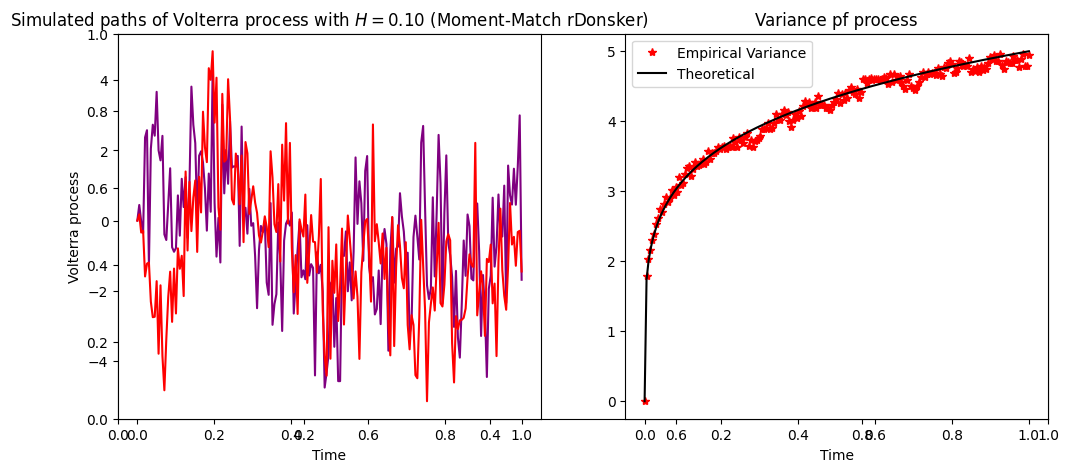
\includegraphics[scale=0.6]{volterra.png}
        \caption{Gaussian Volterra process via rDonsker approximation}
        \label{fig:first}
\end{figure}

\subsubsection{Variance and log-price processes}
The rough Bergomi model is simulated in two stages. We first evaluate the variance process from the simulated Volterra process, and then simulate the log-price by a classical Euler scheme. The first stage amounts to evaluating the stochastic exponential $\mathcal{E}(\cdot)$ of equation \ref{var rb}. Recall that,  the stochastic exponential is defined as
$\mathcal{E}(A_t)=\exp\left(A_t-\frac{1}{2}[A]_t\right)$.
Let the discretization of $(\mathcal K\cdot W)_t$ in Equation~\ref{discretization} be denoted by \({Y}_t\). Then
\[
\mathcal E\left(\sqrt {2H}\nu\,(\mathcal K\cdot W)_t\right)=\exp\left(\sqrt{2H}\nu Y_t-\frac{1}{2}\nu^2t^{2H}\right),
\]
where $\displaystyle \left[\sqrt{2H}\nu\,(\mathcal K\cdot W)\right]_t=2H\nu^2\int_0^t(t-s)^{2H-1}ds=\nu^2t^{2H}$ is its quadratic variation.\vspace{1em}\\
Computing $V_t$ explicitly and, by means of the Euler scheme for the log-price with correlated Brownian motion $B_t=\rho W_t+\sqrt{1-\rho^2}\,Z_t$, i.e.
\[
X_{t_{k+1}}=X_{t_k}-\frac{1}{2}V_{t_k}d t+\sqrt{V_{t_k}}\,\Delta B_{t_k},
\]
we retrieve the model simulation, yielding the variance and log-price paths $\{(V_t^{(i)})_{t\in[0,T]},\,X_T^{(i)}\}_i$ that drive the pricing below.\vspace{1em}\\
\subsection{Pricing and implied-volatility surfaces}\label{implied vol generation chapter}
With the underlying paths in hand, we now price the relevant payoffs: vanilla European calls, which we invert to implied volatilities, and down-and-out digital barriers.
\subsubsection{Vanilla call}
\textit{Pricing problem.} The price of a European call is the discounted expected payoff $\mathbb{E}\!\left[(S_0e^{X_T}-K)^+\right]$, which the standard Monte Carlo estimator approximates by averaging the payoff over the simulated paths. For rough models this estimator suffers from high variance; most visibly, for deep in-the-money strikes it frequently violates the arbitrage bound $C\geq(S_0-K)^+$. To control this, Horvath et al.~\cite{2} apply a variance-reduction scheme that conditions on the variance-driving Brownian motion and prices each path in closed form via Black--Scholes.

\textit{Variance reduction.} Let $
dX_t = -\frac{1}{2}V_t\,dt + \sqrt{V_t}\,dB_t$
and  $B_t = \rho W_t + \sqrt{1-\rho^2}Z_t$. We rewrite the SDE as
\begin{align*}
dX_t &= -\frac{1}{2}V_t\,dt + \sqrt{V_t}\left(\rho\,dW_t + \sqrt{1-\rho^2}\,dZ_t\right)\\
dX_t &= \underbrace{\left(-\frac{1}{2}\rho^2 V_t\,dt + \rho\sqrt{V_t}\,dW_t\right)}_{dX_t^{||}} + \underbrace{\left(-\frac{1}{2}(1-\rho^2)V_t\,dt + \sqrt{1-\rho^2}\sqrt{V_t}\,dZ_t\right)}_{dX_t^{\perp}}
\end{align*}
Integrating over $[0,T]$,
\begin{align*}
X_T^{||} &= -\frac{1}{2}\rho^2\int_0^T V_t\,dt + \rho\int_0^T\sqrt{V_t}\,dW_t \\[6pt]
X_T^{\perp} &= -\frac{1}{2}(1-\rho^2)\int_0^T V_t\,dt + \sqrt{1-\rho^2}\int_0^T\sqrt{V_t}\,dZ_t\end{align*}
$\Rightarrow X_T = X_T^{||} + X_T^{\perp}$. We then condition on $\mathcal{F}^W_T$. $X_T^{||}$ is deterministic, while $X_T^{\perp}|\mathcal{F}^W_T$ is Gaussian, $\displaystyle
X_T^{\perp}\,|\,\mathcal{F}^W_T \;\sim\; \mathcal{N}\!\left(-\frac{1}{2}(1-\rho^2)\int_0^T V_t\,dt,\;\; (1-\rho^2)\int_0^T V_t\,dt\right)$.

\[\Rightarrow 
X_T\,|\,\mathcal{F}^W_T \;\sim\; \mathcal{N}\!\left(X_T^{||} - \frac{1}{2}\underbrace{(1-\rho^2)\int_0^T V_t\,dt}_{\sigma^2},\;\; \underbrace{(1-\rho^2)\int_0^T V_t\,dt}_{\sigma^2}\right)
\]
Therefore $e^{X_T}|\mathcal{F}^W_T$ is log-normal with forward $S_0 e^{X_T^{||}}$ and variance $\sigma^2$. The Black--Scholes formula applies: $
\mathbb{E}\!\left[\max\!\left(S_0 e^{X_T} - K,\,0\right)\Big|\mathcal{F}^W_T\right] = BS\!\left(S_0 e^{X_T^{||}},\,K,\,T,\,\frac{\sigma}{\sqrt{T}}\right)$. The correspondence between the general solution of Feynman--Kac and this conditional expression is guaranteed by the tower property $
\mathbb{E}\!\left[\max\!\left(S_0 e^{X_T} - K,\,0\right)\right] = \mathbb{E}\!\left[\mathbb{E}\!\left[\max\!\left(S_0 e^{X_T} - K,\,0\right)\Big|\mathcal{F}^W_T\right]\right]$.
In effect, the implementation replaces the standard Monte Carlo payoff averaging with a Black--Scholes evaluation per $W$ path.

\textit{Implied-volatility inversion.} Once a price has been generated for a strike--maturity pair $(K,T)$ and parameter combination $(\xi_0,\nu,\rho,H)$, we recover the implied volatility $\sigma_{\mathrm{BS}}(K,T)$ introduced in Section~\ref{deep calibration chapter} by inverting the Black--Scholes formula. For this project the inversion is solved with the bisection root-finding method, i.e.
\[
\sigma_{\mathrm{BS}}
=
\operatorname{root}_{\sigma\in[\sigma_{\min},\sigma_{\max}]}
\left(C_{\mathrm{BS}}(\sigma)-C_{\mathrm{simul}}\right).
\]
The implementation has also been forced to satisfy the classical no-arbitrage bounds for European call options, such as $C\geq(S_0-K)^+$.

\textit{Dataset.} The procedure above maps a single parameter vector $\theta=(\xi_0,\nu,\rho,H)$ to a single implied-volatility surface. To learn this map we require many such pairs, so we draw $N=80000$ parameter vectors by independent uniform sampling over the box
\[
\xi_0\in[0.01,0.16],\quad
\nu\in[0.3,4],\quad
\rho\in[-0.95,-0.1],\quad
H\in[0.025,0.5].
\]
The box is restricted to negative $\rho$ and small $H$ to reflect the stylised facts of equity-index volatility, namely the leverage effect and the empirically rough regime $H\approx0.1$. Each sampled $\theta$ is priced on the fixed strike--maturity grid
\begin{align*}
&\text{Strikes}
=
\{0.5,0.6,0.7,0.8,0.9,1.0,1.1,1.2,1.3,1.4,1.5\},\\
&\text{Maturities}
=
\{0.1,0.3,0.6,0.9,1.2,1.5,1.8,2.0\},
\end{align*}
yielding an $8\times11=88$-point surface. The resulting dataset of parameter--surface pairs $\{(\theta^{(j)},\sigma^{(j)})\}_{j=1}^{80000}$ thus belongs to $\mathbb{R}^{80000\times (4+88)}$ and forms the input--output data on which the FNN is trained and tested. Figure~\ref{fig:surfaces} shows four volatility surfaces corresponding to four different parameter combinations in the dataset.




\begin{figure}[H]
\begin{center}
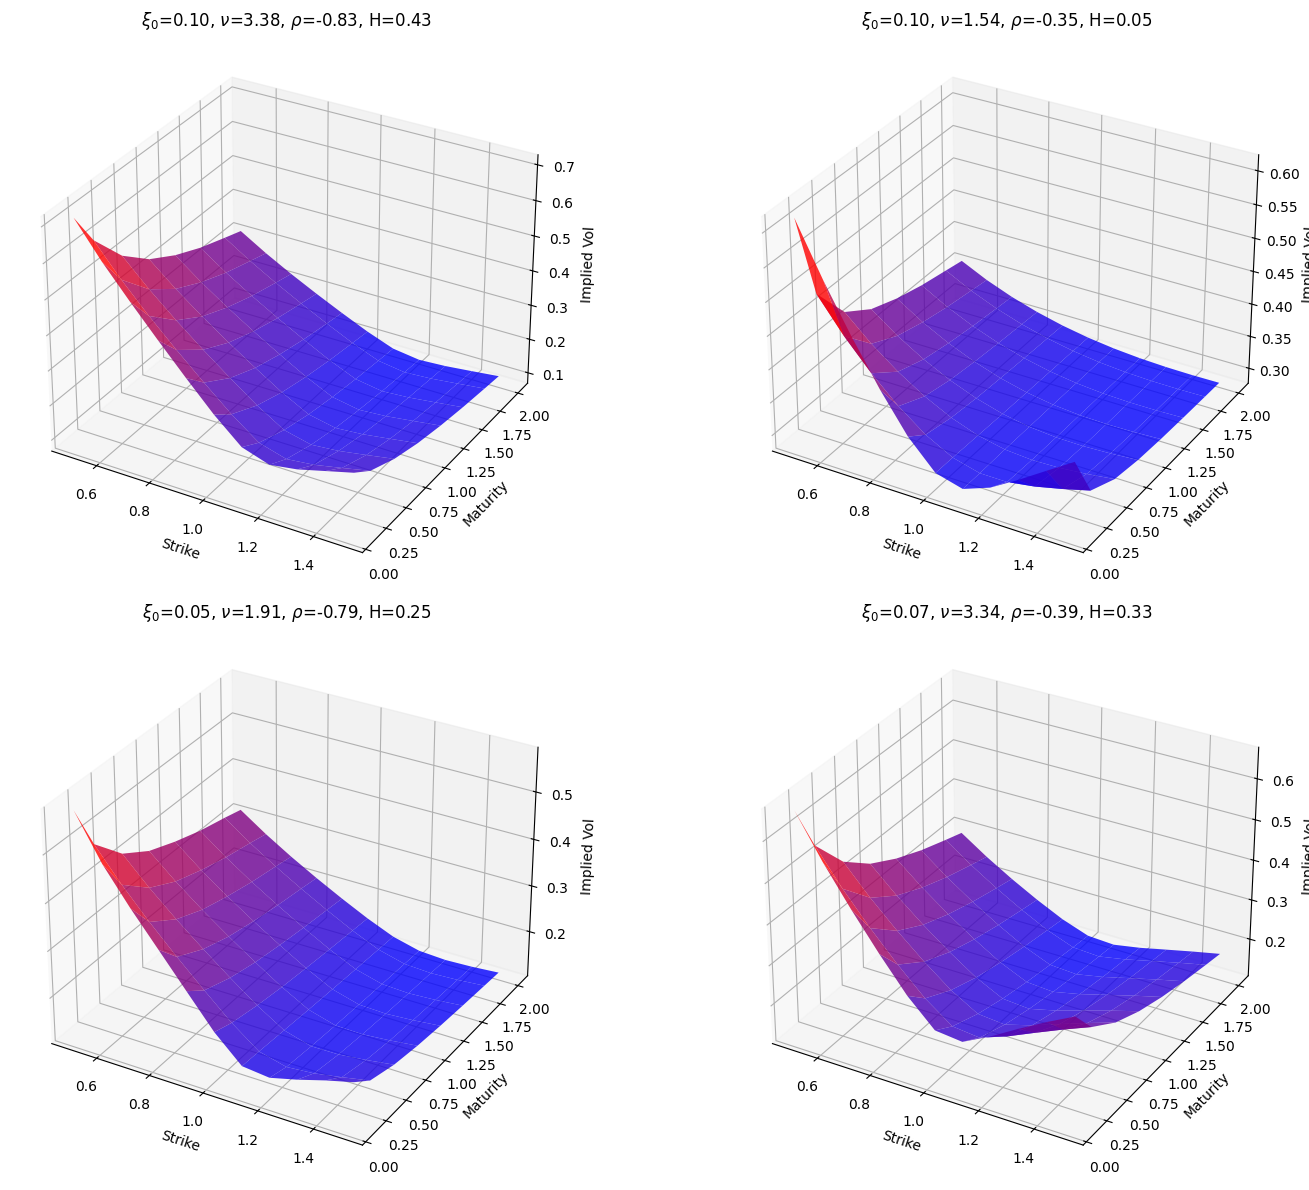
\includegraphics[scale=0.4]{surfaces IV.png}\\
\caption{Volatility surfaces } \label{fig:surfaces}
\end{center}
\end{figure}
\subsubsection{Barrier}
In parallel to the European call, we price a down-and-out (DO) digital barrier with lower barrier $\mathcal B$. Between grid points the discretised path may cross the barrier even when both endpoints lie above it; Glasserman~\cite{glasserman} corrects for this by weighting each path by the Brownian-bridge probability of \emph{no} crossing. Over $[t_i,t_{i+1}]$ with local variance approximated by $V_{t_i}\,dt$ and endpoints $X(t_i),X(t_{i+1})>\log\mathcal B$, this probability is
\[
\hat p_i = 1-\exp\!\left(-\frac{2\,(X(t_i)-\log\mathcal B)\,(X(t_{i+1})-\log\mathcal B)}{V_{t_i}\,dt}\right),
\]
and $\hat p_i = 0$ if either endpoint lies below $\log\mathcal B$. The down-and-out price is then the expected product of these survival probabilities, with the down-and-in following by in--out parity:
\[
\mathrm{DO}(\theta) = \mathbb{E}\!\left[\prod_{i=0}^{n-1}\hat p_i\right],
\qquad
\mathrm{DI}(\theta) = 1-\mathrm{DO}(\theta).
\]
\subsection{The Monte Carlo error floor}\label{mc floor section}
The surfaces used to label the training set are Monte Carlo estimates, so each entry carries sampling noise. This noise imposes an \emph{error floor} on the entire procedure as the network cannot be more accurate than the data from which it learns. This is precisely the target $\widetilde F=\widetilde P+\mathcal O(\epsilon)$ introduced in Section~\ref{deep calibration chapter}. We quantify the floor by the relative half width of the $95\%$ Monte Carlo confidence interval on each implied volatility, reported across the grid in the same format as the network error of Section~\ref{results section} so that the two are directly comparable.

\textit{Standard error in volatility units.} Each Monte Carlo call price $C$ is a path average and carries a standard error $\mathrm{SE}_C$. Since the network is trained on implied volatilities rather than prices, this error must be transported to the volatility scale. We invert both endpoints of the $95\%$ price interval $[\,C-1.96\,\mathrm{SE}_C,\;C+1.96\,\mathrm{SE}_C\,]$ through the Black--Scholes map of Section~\ref{deep calibration chapter} and take half of the resulting spread,
\[
\mathrm{SE}_\sigma
=
\frac{\sigma_{\mathrm{BS}}\!\left(C+1.96\,\mathrm{SE}_C\right)-\sigma_{\mathrm{BS}}\!\left(C-1.96\,\mathrm{SE}_C\right)}{2\times 1.96}.
\]
The floor at a grid point $(T,k)$ is the corresponding relative half width,
\[
\mathrm{floor}_{T,k}=\frac{1.96\,\mathrm{SE}_\sigma}{\sigma_{\mathrm{BS}}(T,k)}.
\]
Averaged over the dataset the floor is $1.23\%$, with a median of $0.57\%$. Figure~\ref{fig:mcfloor} displays its mean and standard deviation across the grid.

\begin{figure}[H]
\begin{center}
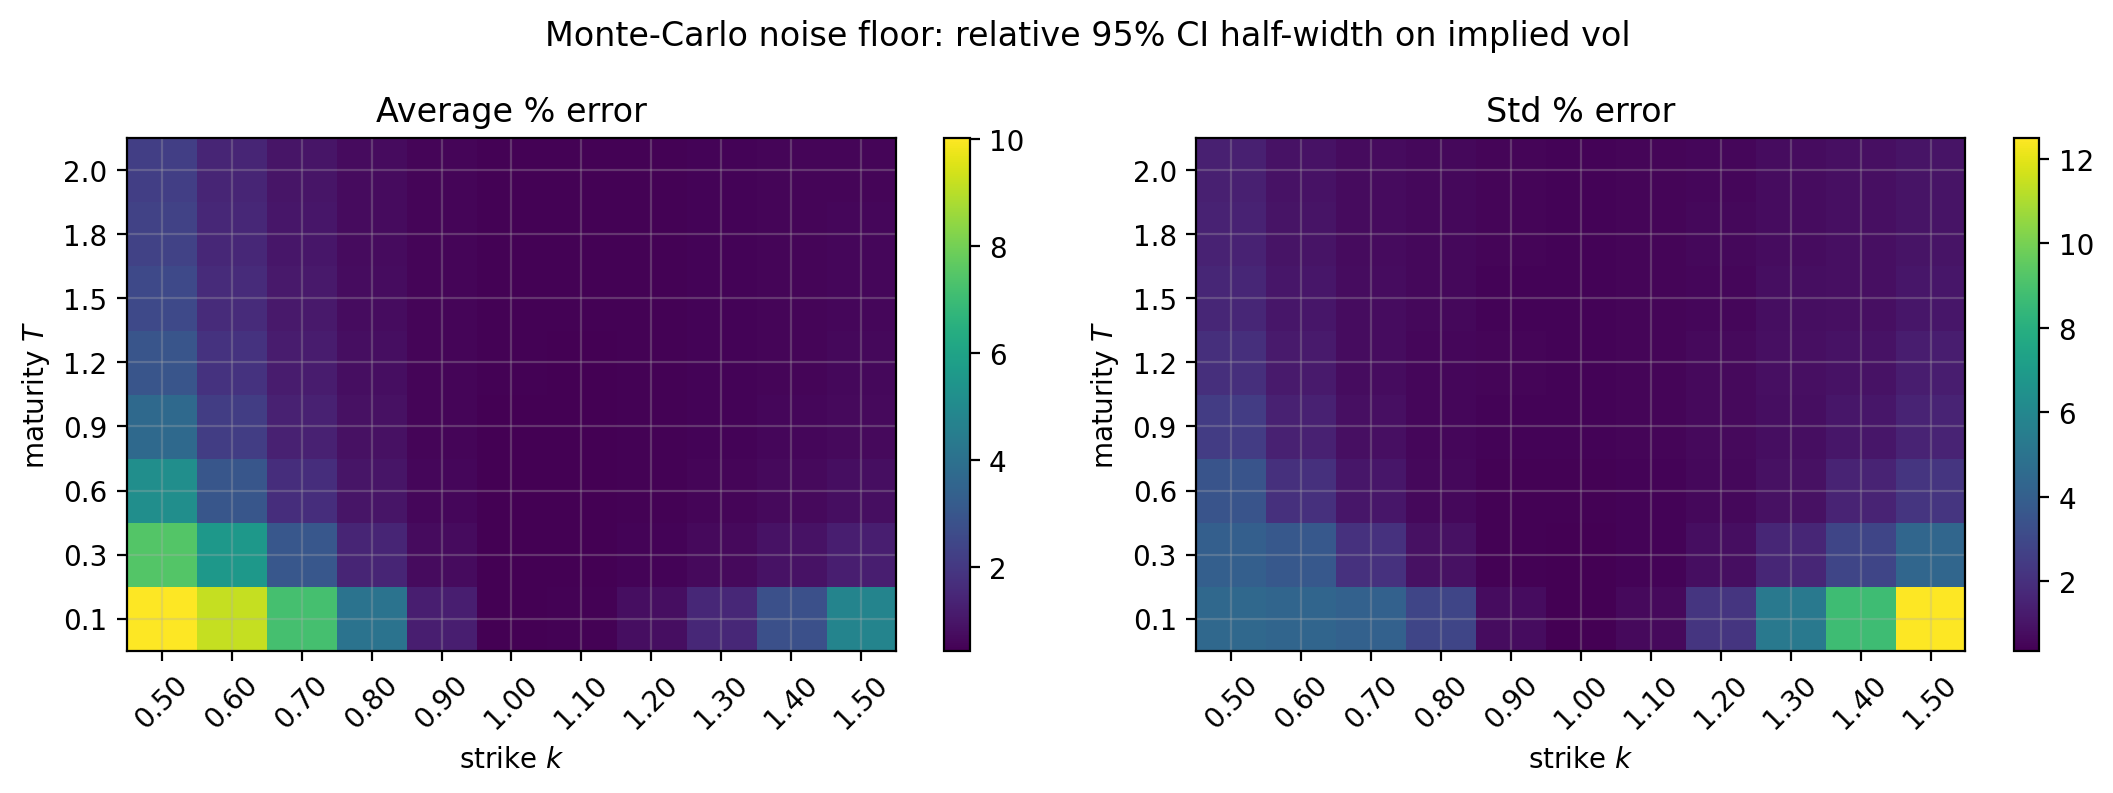
\includegraphics[width=\linewidth]{mc_floor.png}\\
\caption{Monte Carlo error floor: mean and standard deviation of the relative $95\%$ confidence interval half width on the implied volatility, across the $8\times 11$ strike and maturity grid.}
\label{fig:mcfloor}
\end{center}
\end{figure}

The floor is largest in the wings, at short maturities and extreme strikes, where the option has little time value and hence small vega, so price noise is magnified once expressed in volatility units, $\mathrm{SE}_\sigma\approx\mathrm{SE}_C/\mathrm{vega}$.
\subsection{Neural-network training}\label{FNN construction chapter}
\subsubsection{Train/Test split}
We split the $80{,}000$ parameter--surface pairs once: $85\%$ ($68{,}000$ pairs) form the training set and the remaining $15\%$ ($12{,}000$ pairs) a held-out test set. Each pair has a parameter vector in $\mathbb R^4$ as feature and a surface in $\mathbb R^{88}$ as label.

The training set fixes the network weights through the empirical-risk minimisation of Section~\ref{deep calibration chapter},
\[
\widehat w=\operatorname*{argmin}_{w}\widehat R_{N}\!\left(F(\cdot,w)\right),\qquad
\widehat R_{N}(F)=\frac1N\sum_{j=1}^N\big\lVert F(\theta^{(j)})-\sigma^{(j)}\big\rVert_2^2 .
\]
The test set fixes how we measure it. Because the same data both fit and score the weights, the training risk $\widehat R_N$ underestimates the true generalisation risk $R(F)=\mathbb E\lVert F(\theta)-\sigma\rVert_2^2$. The held-out test risk $\widehat R_{\text{test}}$ does not share this bias, so we monitor it throughout training and report final performance on it (Section~\ref{results section}).
\subsubsection{Normalisation}
Both features and labels are normalised before training. Each parameter $\theta=(\xi_0,\nu,\rho,H)$ is mapped component-wise to $[-1,1]$ by the affine transform $\theta\mapsto\big(2\theta-(\theta_{\min}+\theta_{\max})\big)/(\theta_{\max}-\theta_{\min})$, using the box bounds of Section~\ref{implied vol generation chapter}. The surface labels are standardised to zero mean and unit variance with \texttt{StandardScaler}, fit on the training labels alone and applied to both sets; predictions are returned to volatility units by inverting the transform.
\subsubsection{Network architecture}
The network is the class $\mathcal N\mathcal N_5(4,30,30,30,30,88,\, \mathrm{ELU}, \mathrm{ELU}, \mathrm{ELU}, \mathrm{ELU}, \mathrm{id})$: an input of dimension $4$, four hidden layers of $30$ units with ELU activation, and a linear output layer of dimension $88$. Algorithm~\ref{alg:ffn} gives the forward pass.




\begin{algorithm}[H]
\caption{Feed-forward neural network architecture}
\label{alg:ffn}
\begin{algorithmic}[1]

\State \textbf{Input:} Parameter vector
$\theta=(\xi_0,\nu,\rho,H)\in\mathbb{R}^4$

\State \textbf{Output:} Predicted implied volatility surface
$\widetilde{F}(\theta)\in\mathbb{R}^{88}$

\State Define the input layer with dimension $4$
\State $x_1 \gets \operatorname{ELU}\!\left(W_1\theta+b_1\right)$,
\quad $x_1\in\mathbb{R}^{30}$
\State $x_2 \gets \operatorname{ELU}\!\left(W_2x_1+b_2\right)$,
\quad $x_2\in\mathbb{R}^{30}$
\State $x_3 \gets \operatorname{ELU}\!\left(W_3x_2+b_3\right)$,
\quad $x_3\in\mathbb{R}^{30}$
\State $x_4 \gets \operatorname{ELU}\!\left(W_4x_3+b_4\right)$,
\quad $x_4\in\mathbb{R}^{30}$
\State $\widetilde{F}(\theta)\gets W_5x_4+b_5$,
\quad $\widetilde{F}(\theta)\in\mathbb{R}^{88}$
\State Compile the model using the mean squared error loss
\State Optimise the network parameters using the Adam optimiser

\end{algorithmic}
\end{algorithm}
for a total of $(4\times 30+30)+3\times(30\times30+30)+(30\times 88+88)=5668$ weights and biases. Two of these choices are deliberate.

\textbf{Activation.} We use ELU rather than ReLU because $\sigma_{\mathrm{ELU}}\in C^1(\mathbb R)$. By the universal approximation theorem for derivatives of Section~\ref{neural networks section}, this lets the network approximate not only $F^*$ but also its gradient, $\nabla_\theta\widetilde F\approx\nabla_\theta F^*$, the smoothness on which the gradient-based calibration of Section~\ref{calibration chapter} relies. A non-differentiable choice such as ReLU would not provide it.

\textbf{Depth.} The four hidden layers follow the original architecture \cite{1}, beyond which no material gain is observed for this map.

Figure~\ref{fig:nnarch} shows the resulting architecture.
\begin{figure}[H]
\begin{center}
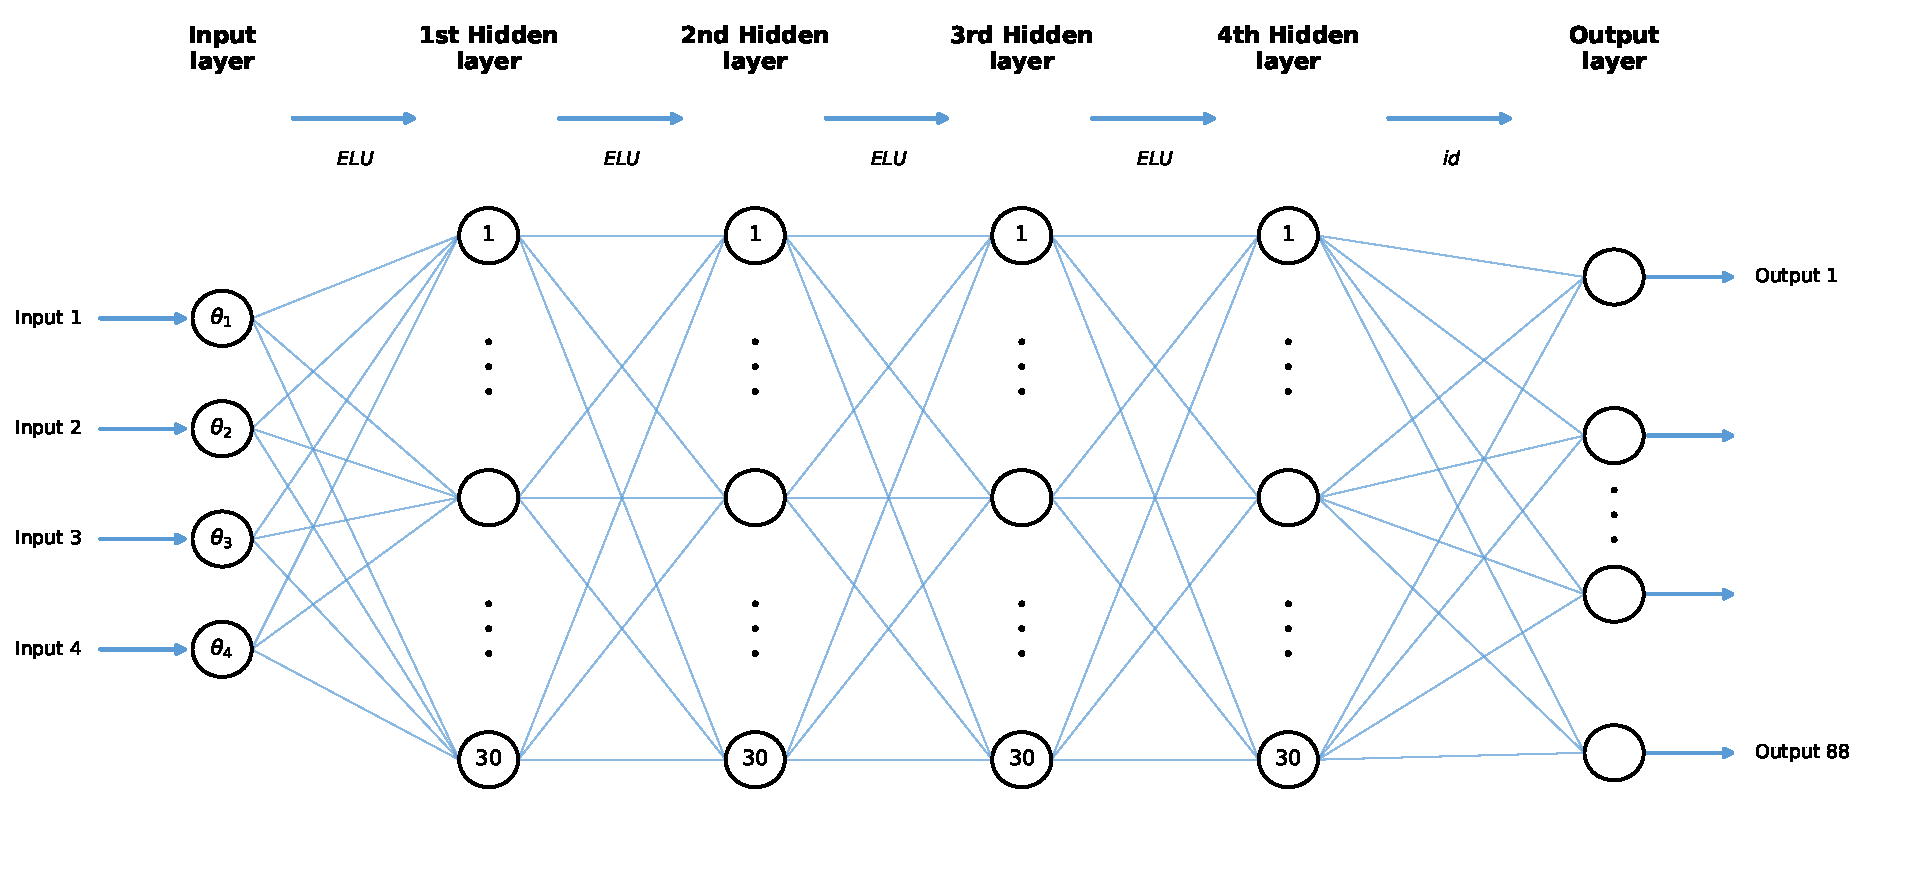
\includegraphics[width=\linewidth]{nn_architecture.pdf}\\
\caption{Neural Network structure } \label{fig:nnarch}
\end{center}
\end{figure}
\subsubsection{Training}
We minimise the empirical risk $\widehat R_N$ over the weights $w$ with the Adam optimiser, a mini-batch stochastic gradient descent scheme, using batch size $32$ and a budget of $200$ epochs. After each epoch we record both the training risk and the test risk $\widehat R_{\text{test}}$, the unbiased estimator of the generalisation risk from Section~\ref{FNN construction chapter}.

Early stopping regularises the fit: training halts once $\widehat R_{\text{test}}$ has not improved for $25$ consecutive epochs, and the weights are restored to those of the best epoch. This guards against overfitting, the regime in which the training risk keeps falling while the test risk has flattened.

Figure~\ref{fig:risk} shows the two risks over training. They descend together and plateau jointly, with no widening gap, indicating that the network generalises rather than memorises and that the stopping point is well chosen.

\begin{figure}[H]
\begin{center}
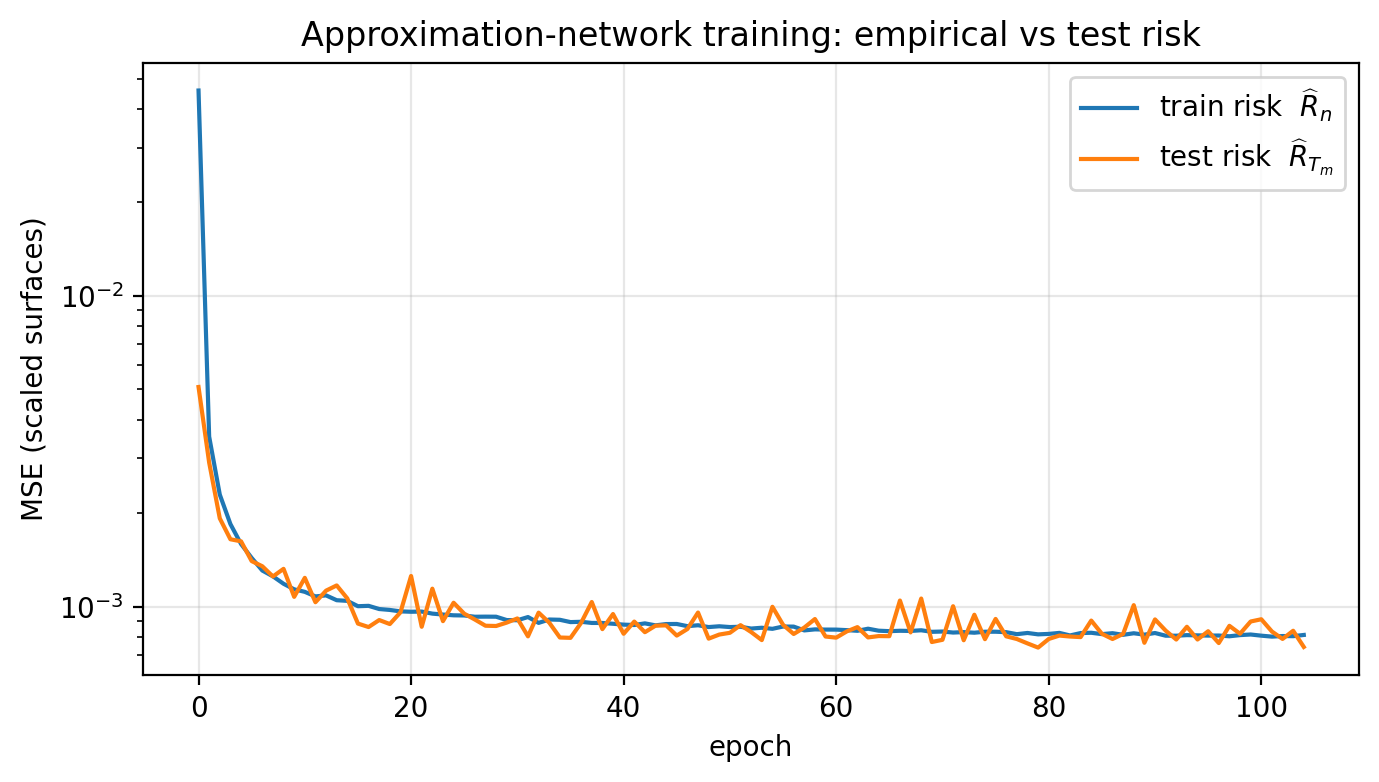
\includegraphics[scale=0.9]{emp_risk_vstest.png}\\
\caption{Training and test risk over epochs (MSE on the scaled surfaces, log scale).} \label{fig:risk}
\end{center}
\end{figure}
\subsection{Results}\label{results section}
With the weights frozen, we evaluate the trained map on the $12000$ held-out test surfaces and compare its outputs against the Monte Carlo labels. Figure~\ref{figerror} reports the relative implied-volatility error per grid point, in the same two-panel format (mean and standard deviation) as the Monte Carlo floor of Figure~\ref{fig:mcfloor} so that the two are read side by side, while Figure~\ref{fig:smilefit} shows the fitted smiles for the best- and worst-fit test surfaces.
\begin{figure}[H]
\begin{center}
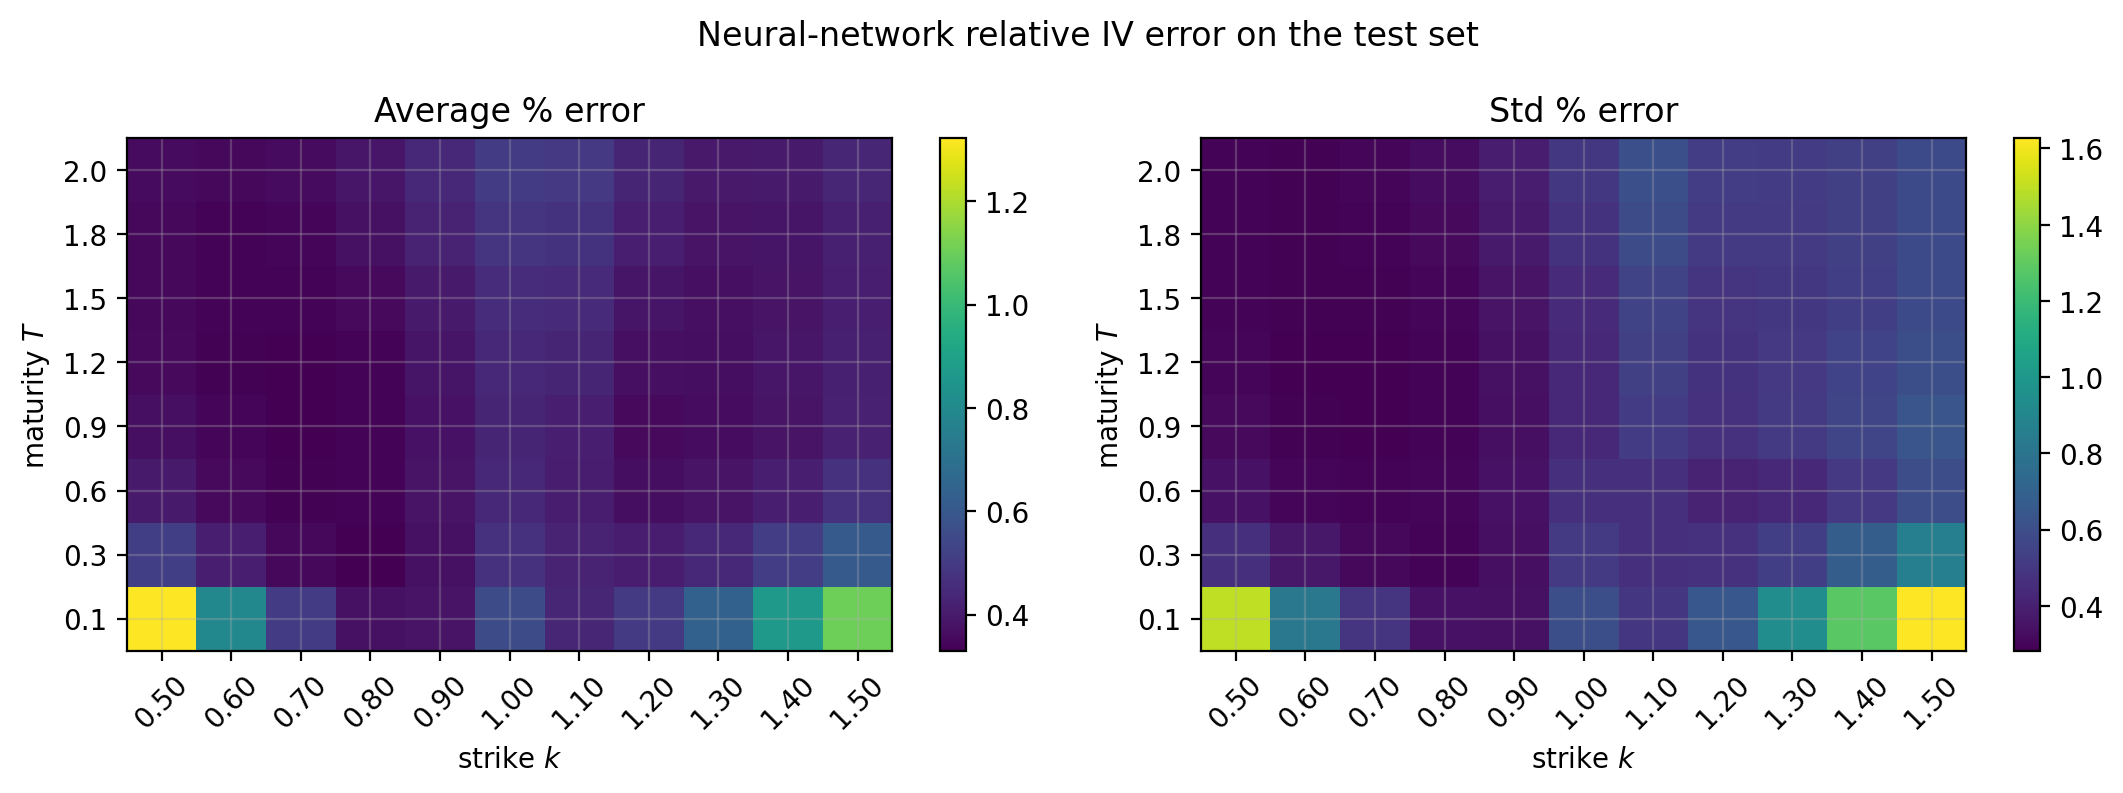
\includegraphics[width=\linewidth]{NN_error.png}\\
\caption{Neural-network relative implied-volatility error on the test set: mean and standard deviation across the $8\times11$ grid.} \label{figerror}
\end{center}
\end{figure}
\begin{figure}[H]
\begin{center}
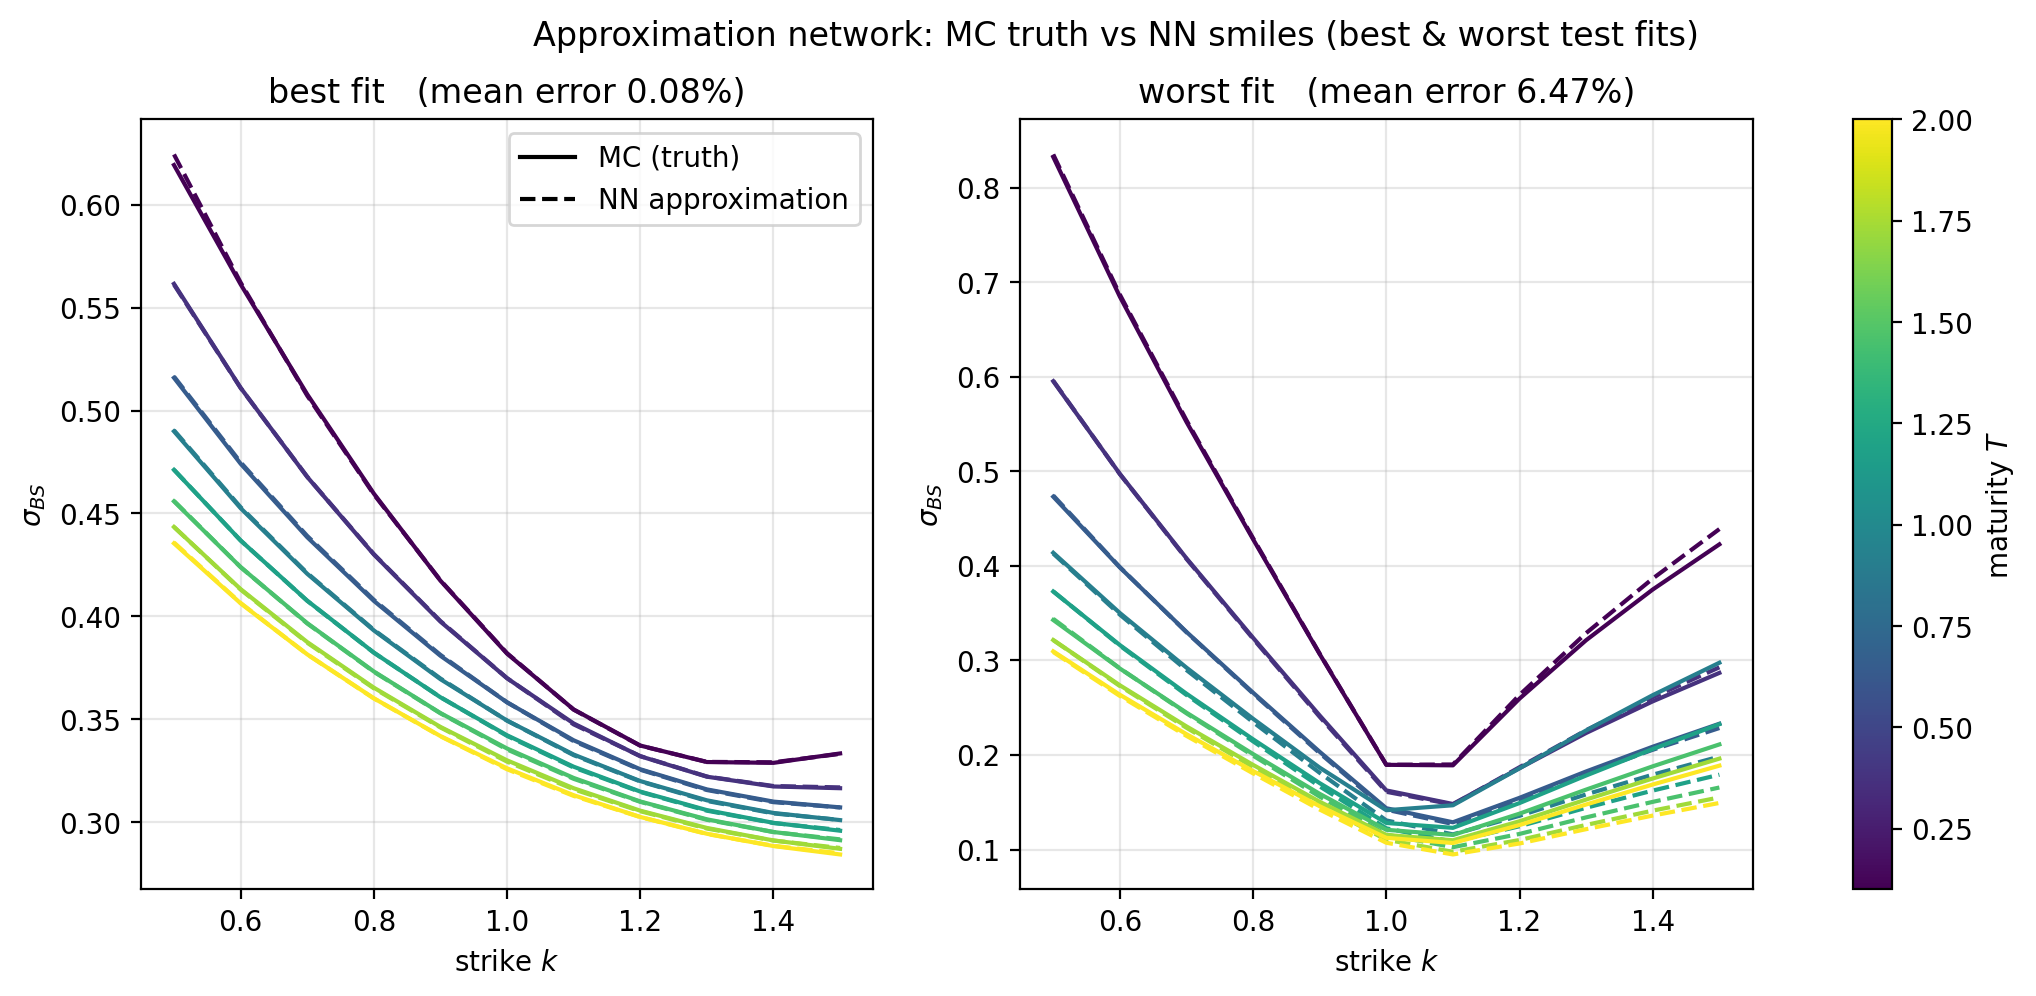
\includegraphics[width=\linewidth]{smiles.png}\\
\caption{Monte Carlo prices against the neural-network approximation for the best- and worst-fit test surfaces.} \label{fig:smilefit}
\end{center}
\end{figure}
The network attains a mean relative implied-volatility error of $0.43\%$ on the test set (Figure~\ref{figerror}). This is small in practical terms: it lies below a typical bid-ask spread, reported by Horvath et al.~\cite{1} as about $0.2\%$ in volatility terms, roughly $1\%$ in relative terms, for liquid options under one year. The approximation is therefore well within the tolerance needed to calibrate to market data. 

The error is also of the same order as the Monte Carlo sampling floor of $1.23\%$ (Section~\ref{mc floor section}), so the network is about as accurate as the data it was trained on. The largest residuals occur at short maturities and at the extreme strikes, where the options carry little time value and the implied volatility is hardest to pin down. Figure~\ref{fig:smilefit} shows that even the worst-fit test surface tracks the Monte Carlo smiles closely.










\section{Online calibration}\label{calibration chapter}
This section realises step~(ii) of the framework of Section~\ref{deep calibration chapter}. Section~\ref{approximate pricing map} produced a trained network $\widetilde F$ that returns an implied-volatility surface for any parameter vector at negligible cost. We now use it to calibrate the model. Calibration is the approximate problem~\eqref{approx calibration} with the Monte Carlo pricer $\widetilde P$ replaced by $\widetilde F$. Because $\widetilde F$ is deterministic and differentiable, the optimisation that was intractable under Monte Carlo reduces to a routine least-squares fit. We describe the method (Section~\ref{calib method}), calibrate the network to held-out surfaces with known parameters to measure its accuracy and speed (Section~\ref{calib results}), and compare optimisers to justify our choice (Section~\ref{calib optimisers}).

\subsection{Method}\label{calib method}
\subsubsection{Calibration as least squares}
Given a target surface $\Sigma^{\mathrm{MKT}}_{BS}$, calibration solves
\[
\hat\theta=\operatorname*{argmin}_{\theta\in\Theta}\big\lVert\widetilde F(\theta)-\Sigma^{\mathrm{MKT}}_{BS}\big\rVert_2^2.
\]
We solve it in the scaled coordinates of Section~\ref{FNN construction chapter}, with the parameters mapped to $[-1,1]$ and the surfaces standardised, so that every residual component is on a comparable scale. The optimiser starts from the centre of the parameter box and the recovered vector is returned to model units afterwards. The objective is a sum of squares over the $88$ grid points, the natural form for a least-squares solver.

\subsubsection{An exact gradient from the frozen network}
The fit is gradient-based and therefore requires the Jacobian $\nabla_\theta\widetilde F$. Since the network is an explicit composition of affine maps and the $C^1$ ELU activation, this Jacobian is available in closed form and is evaluated exactly by the chain rule, with no finite differencing. This is the practical payoff of the activation chosen in Section~\ref{neural networks section}: the derivative-approximation guarantee $\nabla_\theta\widetilde F\approx\nabla_\theta F^*$ holds, so the optimiser follows a faithful gradient of the true pricing map. A ReLU network, not being $C^1$, would not provide this.

For speed inside the optimiser loop we evaluate the forward pass and the analytic Jacobian with a lightweight \texttt{NumPy} copy of the trained weights. This copy reproduces the Keras network to machine precision, with a maximum absolute difference of $8.9\times10^{-16}$ on a test input. By contrast, a brute-force Monte Carlo calibration has no closed-form gradient and must approximate it by finite differences, which is both slower and noisier.

\subsubsection{The Levenberg--Marquardt optimiser}
We carry out the fit with the Levenberg--Marquardt algorithm, which is designed for least-squares objectives and uses the residual and its Jacobian directly. The reasons for preferring it to the alternatives are given in Section~\ref{calib optimisers}.

\subsection{Results}\label{calib results}
We assess the calibration on the held-out test surfaces of Section~\ref{results section}. Each test surface was generated from a known parameter vector, so recovering that vector provides a controlled, self-consistent measure of calibration quality.

The procedure is fast. Calibrating $1000$ test surfaces takes $0.37$~ms each on average. Measured against the Monte Carlo pricing cost of Section~\ref{rough bergomi chapter}, this is the order-of-magnitude speed-up that the two-step design is built to deliver, consistent with the speed-ups reported in the original paper.

We report accuracy with two measures: the relative error $|\hat\theta-\theta|/|\theta|$ of each recovered parameter, and the root-mean-square error (RMSE) between the target surface and the surface repriced at $\hat\theta$. The median parameter relative errors are $0.59\%$ for $\xi_0$, $0.65\%$ for $\nu$, $0.91\%$ for $\rho$ and $1.76\%$ for $H$. The surface RMSE has a median of $0.095\%$ and a $99\%$ quantile of $0.438\%$, inside the benchmark $99\%$ quantile of $1\%$ used in the paper. Figure~\ref{fig:calibcdf} shows the empirical distributions of both quantities across the test set.

\begin{figure}[H]
\centering
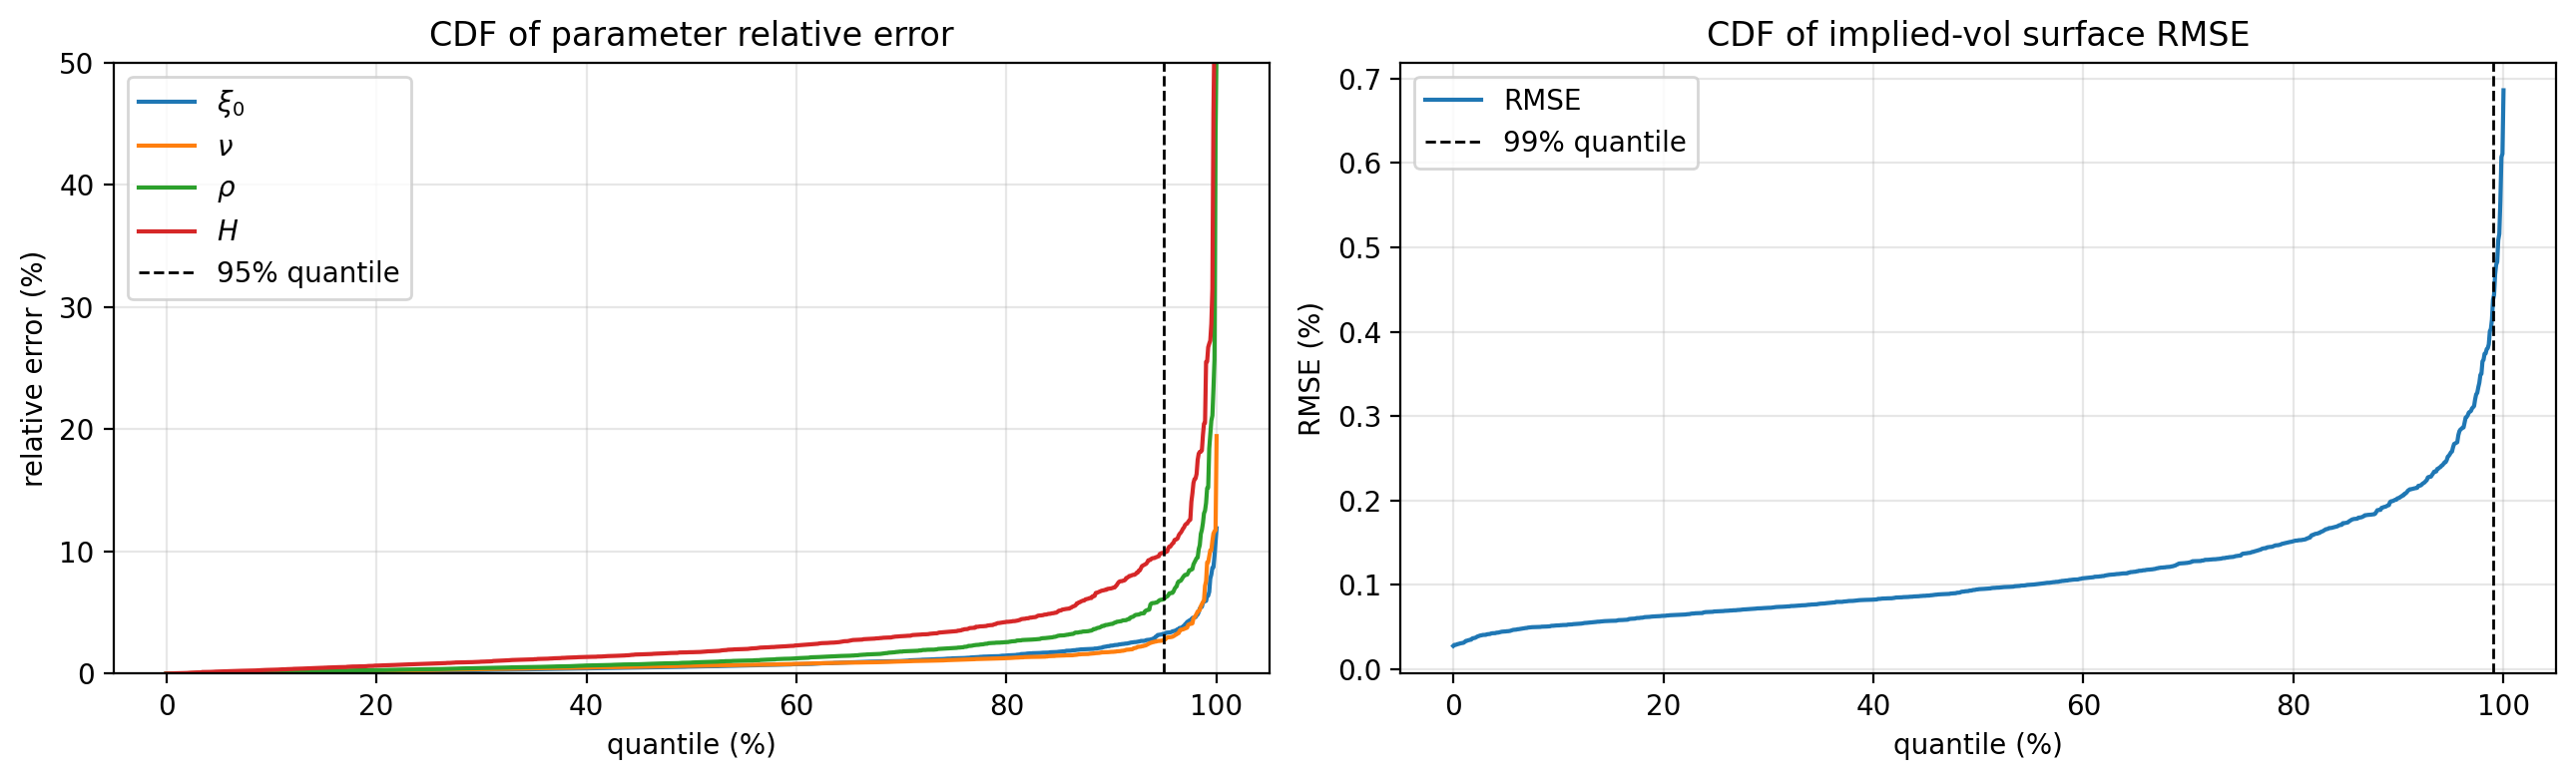
\includegraphics[width=\linewidth]{calib_cdf.png}
\caption{Empirical cumulative distribution functions of the parameter relative error (left, with the $95\%$ quantile marked) and of the implied-volatility surface RMSE (right, with the $99\%$ quantile marked), across the calibrated test surfaces.}
\label{fig:calibcdf}
\end{figure}

The parameter error is not uniform across the parameter space. Figure~\ref{fig:calibscatter} resolves it against the true value, one panel per parameter. The Hurst parameter $H$, and to a lesser extent the correlation $\rho$, are the least identifiable, with the largest errors at small $H$ and at $\xi_0$ near its lower bound. In those regions the surface is least sensitive to the parameter, so a range of values reproduces it almost equally well, and the small denominator further inflates the relative error. This reflects the conditioning of the calibration problem rather than a deficiency of the network.

\begin{figure}[H]
\begin{center}
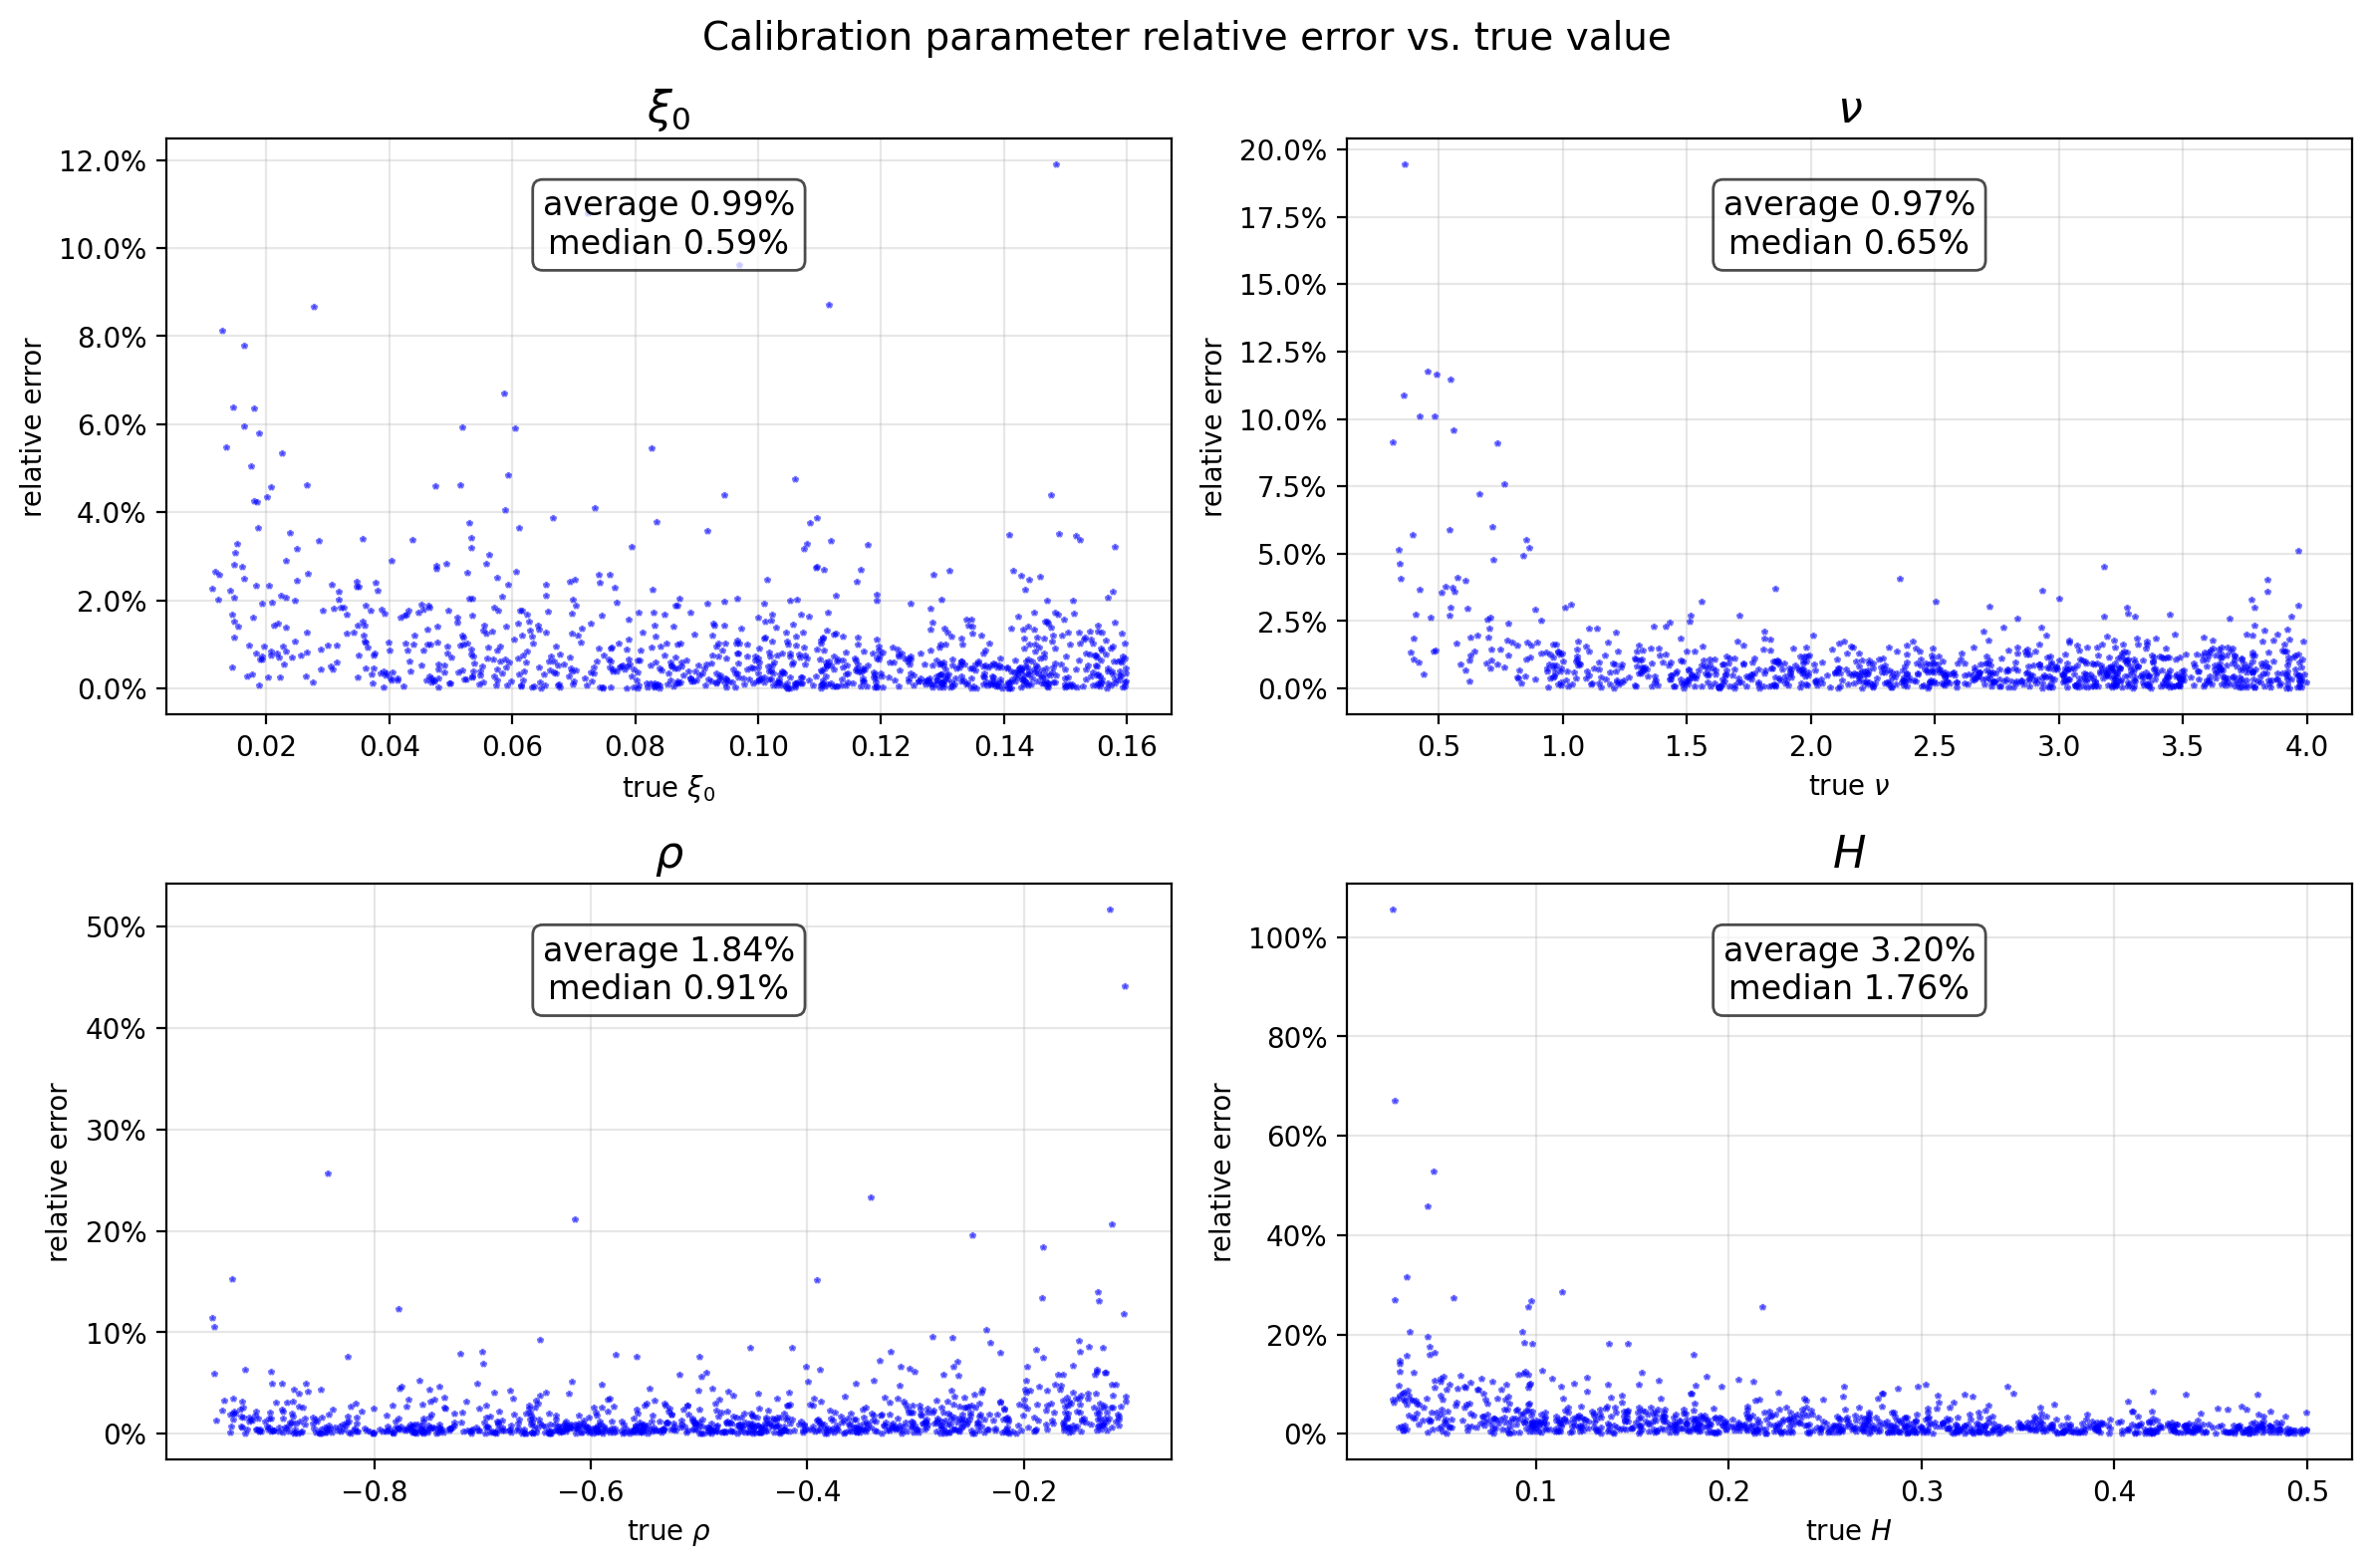
\includegraphics[width=\linewidth]{calib_scatter.png}\\
\caption{Calibration parameter relative error against the true parameter value, one panel per parameter. The error is largest for small $H$ and for $\xi_0$ near its lower bound, where the surface is least sensitive to the parameter.}
\label{fig:calibscatter}
\end{center}
\end{figure}

Read as implied-volatility smiles, the fits are close even in the worst case. Figure~\ref{fig:calibsmiles} shows the best- and worst-fit test surfaces, ranked by mean relative error across the grid; the two mean errors are $0.06\%$ and $1.89\%$. The calibrated smiles track the targets across maturities in both panels.

\begin{figure}[H]
\begin{center}
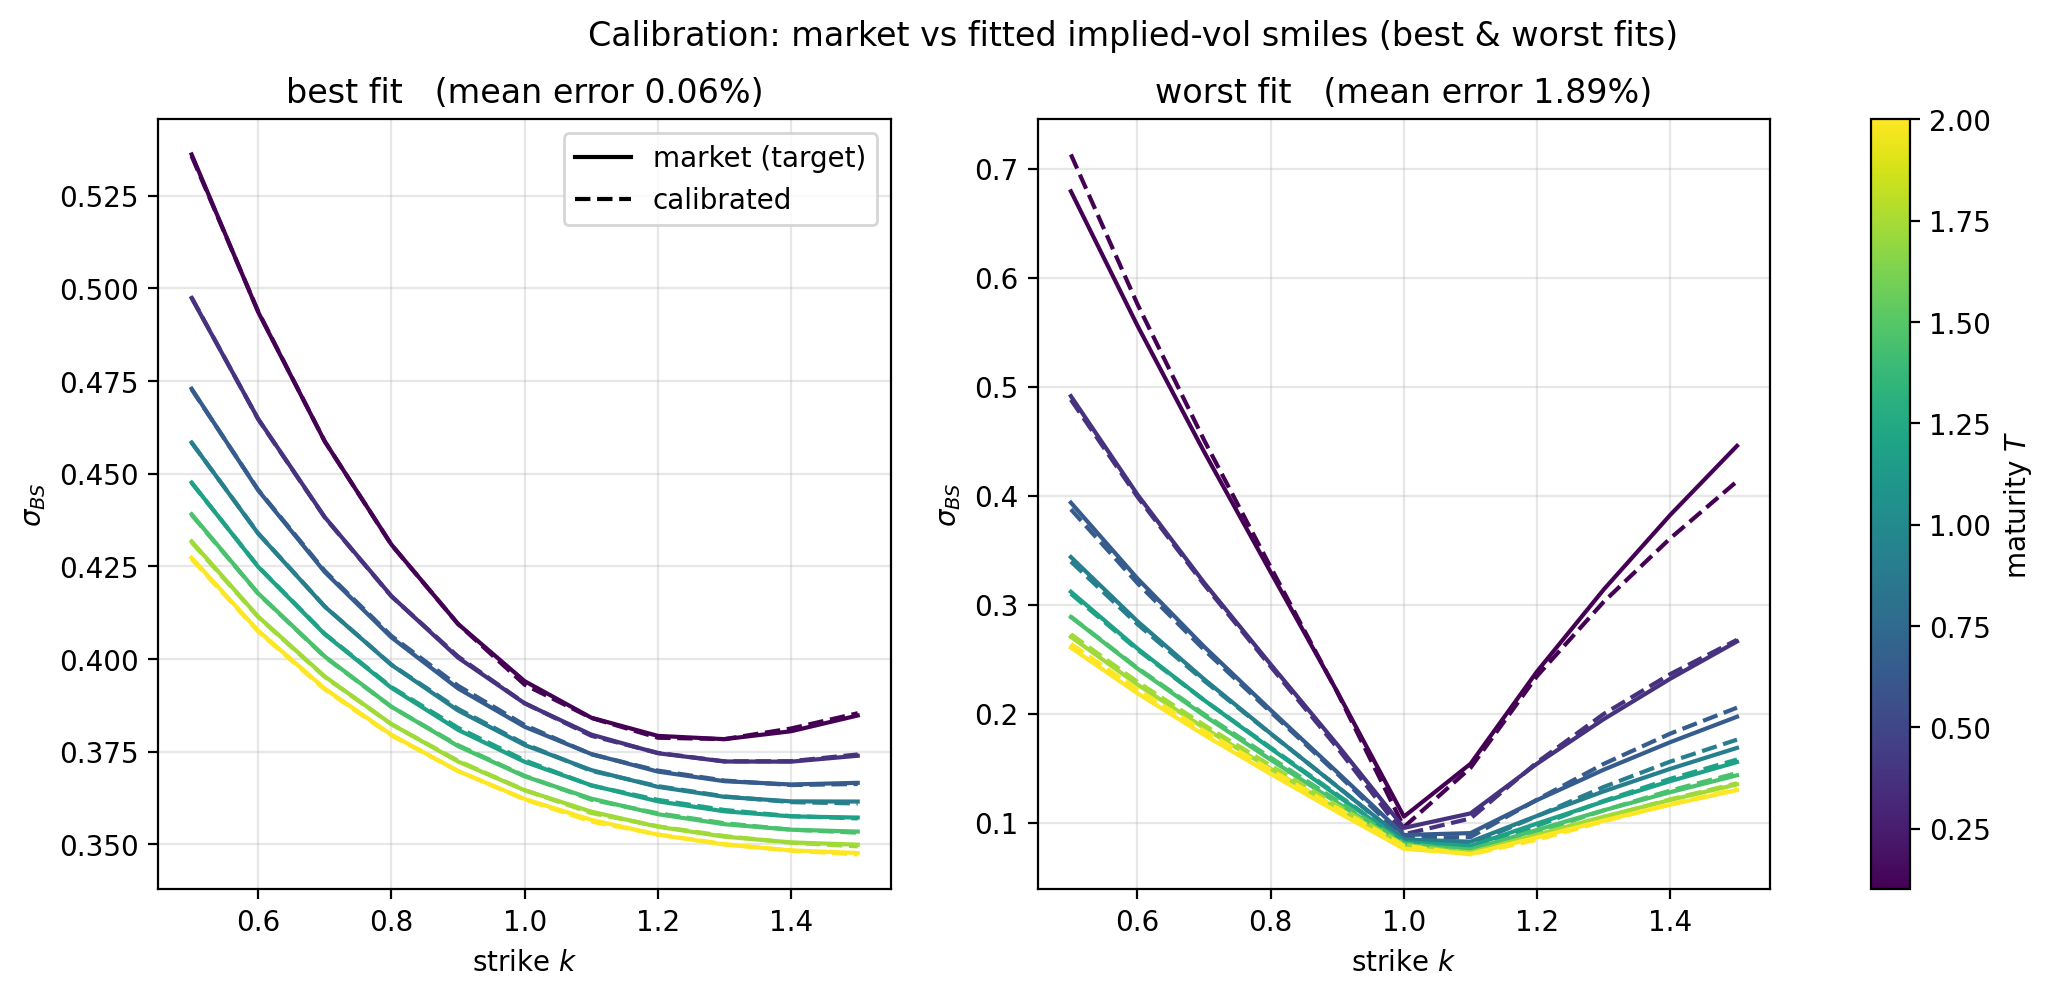
\includegraphics[width=\linewidth]{calib_smiles.png}\\
\caption{Market target against the calibrated surface, read as implied-volatility smiles, for the best- and worst-fit test surfaces. Solid curves are the target, dashed curves the calibrated fit; colour denotes maturity.}
\label{fig:calibsmiles}
\end{center}
\end{figure}

\subsection{Choosing the optimiser}\label{calib optimisers}
Levenberg--Marquardt is one of several optimisers able to solve the frozen-network calibration. We compare seven, in two families (cf. Horvath et al.~\cite{1}, Table~1). The gradient-based methods, Levenberg--Marquardt, BFGS, L-BFGS-B and SLSQP, use the exact Jacobian of Section~\ref{calib method} and converge in few iterations, but rely on the smoothness that the $C^1$ activation provides. The gradient-free methods, Nelder--Mead, COBYLA and Differential Evolution, require no derivatives and can search globally, at the cost of many more function evaluations.

Figure~\ref{fig:calibopt} reports the average calibration time per surface for each optimiser on a logarithmic scale. The gradient-based methods are one to three orders of magnitude faster than the gradient-free ones while reaching the same surface RMSE, around $0.10\%$ in every case. Levenberg--Marquardt is the fastest of all, at $0.36$~ms per surface, which is why we adopt it in Section~\ref{calib results}. This reproduces the paper's finding.

\begin{figure}[H]
\begin{center}
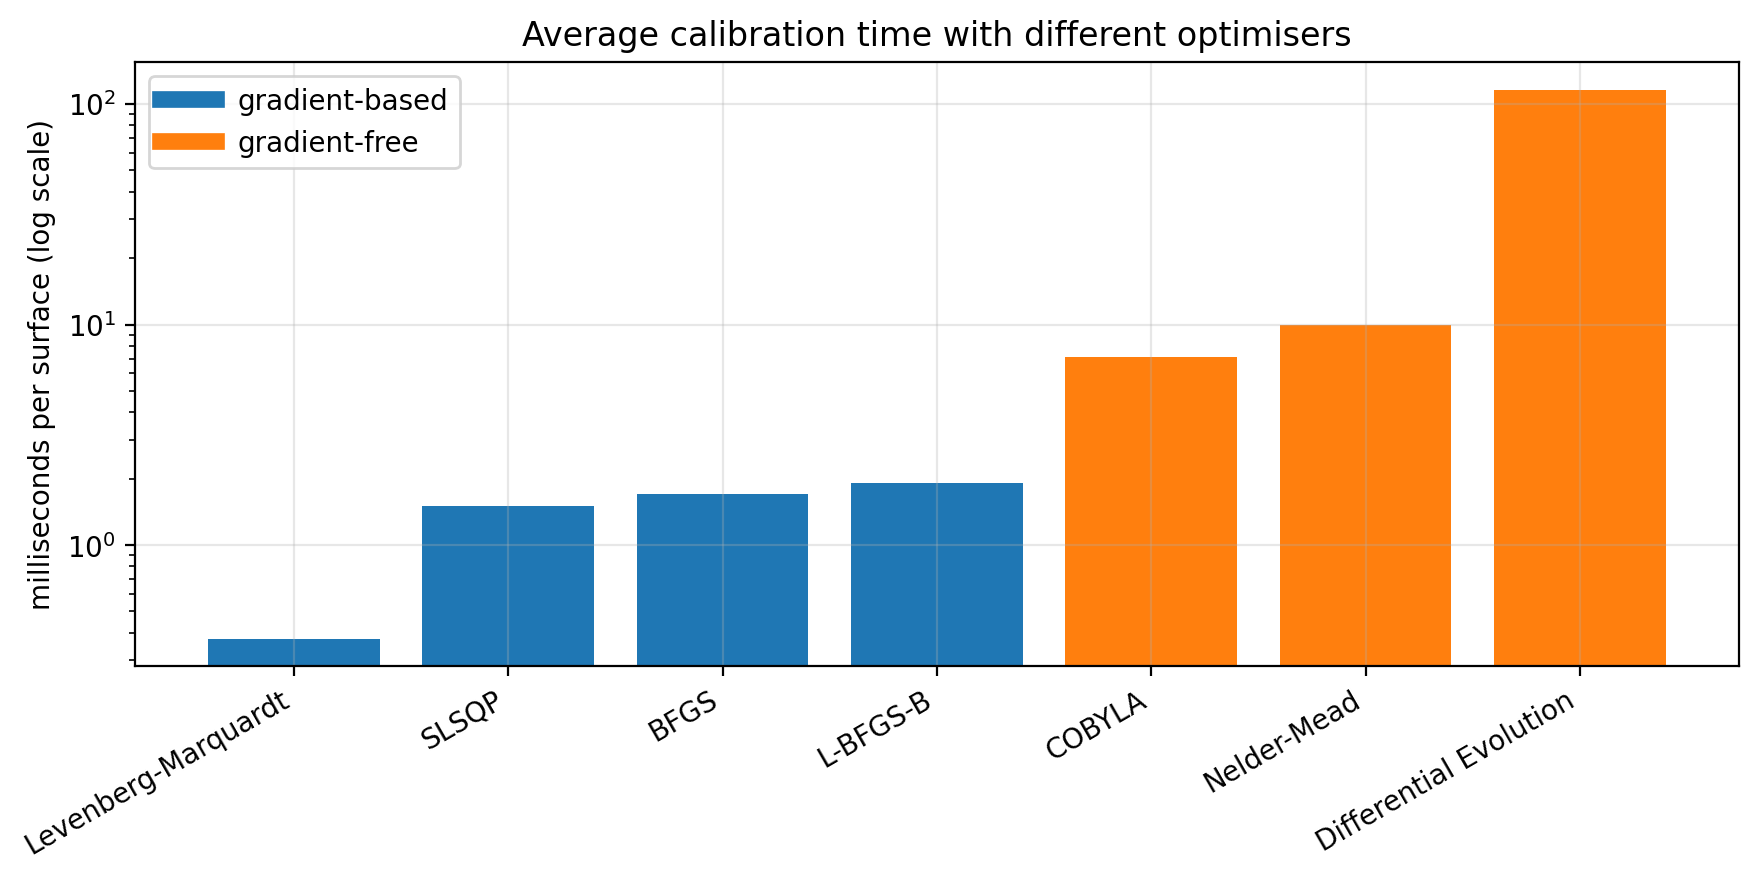
\includegraphics[width=\linewidth]{calib_optimizers.png}\\
\caption{Average calibration time per surface for seven optimisers (log scale). Gradient-based methods (blue) are far faster than gradient-free ones (orange), with Levenberg--Marquardt the fastest.}
\label{fig:calibopt}
\end{center}
\end{figure}

\subsection{Scope and extensions}
We calibrated the rough Bergomi model with a flat forward-variance level to simulated surfaces. Two extensions follow the paper directly. The first is a piecewise-constant forward-variance curve $\xi_0(t)$, with one value per maturity, which adds eight inputs to the network and a realistic term structure. The second is calibration to historical market data: Horvath et al.~\cite{1} calibrate the rough Bergomi model to ten years of SPX implied-volatility surfaces and recover a Hurst parameter $H<1/2$ throughout, in line with the empirical roughness of equity volatility.


\clearpage


\begin{thebibliography}{99}

\bibitem{1} B. Horvath, A. Muguruza, M. Tomas,  \emph{Deep learning volatility: A deep neural network perspective on pricing and calibration in (rough) volatility models} (2021).

\bibitem{2} B. Horvath, A. Jacquier, A. Muguruza, A. S{\o}jmark, 
\emph{Functional central limit theorems for rough volatility} (2024).


\bibitem{gatheral}
J. Gatheral, T. Jaisson, M. Rosenbaum,
\emph{Volatility is rough} (2018).

\bibitem{Pakkanen} M. Bennedsen, A. Lunde, M. S. Pakkanen, \emph{Hybrid scheme for Brownian semistationary processes} (2017).

\bibitem{glasserman}
P. Glasserman,
\emph{Monte Carlo Methods in Financial Engineering} (2004).




\end{thebibliography}


\end{document} 